\documentclass[10pt,twocolumn]{article}

\usepackage[margin=0.72in,columnsep=0.28in]{geometry}
\usepackage{lmodern}
\usepackage[T1]{fontenc}
\usepackage{microtype}
\usepackage{amsmath,amssymb,amsthm}
\usepackage{booktabs}
\usepackage{xcolor}
\usepackage{colortbl}
\usepackage{tcolorbox}
\usepackage{tikz}
\usetikzlibrary{arrows.meta,positioning,calc,decorations.pathreplacing}
\usepackage{pgfplots}
\pgfplotsset{compat=1.18}
\usepackage{enumitem}
\setlist{nosep,leftmargin=1.1em}
\usepackage[hidelinks=false,colorlinks=true,linkcolor=sfblue,citecolor=sfgreen,urlcolor=sforange,bookmarks=true,bookmarksopen=true,bookmarksnumbered=true]{hyperref}

\definecolor{sfblue}{HTML}{1F4E79}
\definecolor{sfgreen}{HTML}{1B7F4E}
\definecolor{sforange}{HTML}{C05621}
\definecolor{sfred}{HTML}{B23A48}
\definecolor{sfgold}{HTML}{F4C56D}
\definecolor{sfpanel}{HTML}{F4F7FB}
\definecolor{sfink}{HTML}{E8EEF6}

\newtheorem{claim}{Claim}
\theoremstyle{definition}
\newtheorem{remark}{Remark}

\hypersetup{
  pdftitle={Notes on a Discrete Laplacian for On-Device Preview},
  pdfauthor={SiliconForest Demo},
  pdfsubject={A short math-heavy LaTeX specimen for Preview.app},
  pdfkeywords={Laplacian, TikZ, pgfplots, Preview}
}

\title{\textcolor{sfblue}{Notes on a Discrete Laplacian}\\[2pt]
\large for On-Device Document Preview}
\author{A. Calder\quad B. Okonkwo\quad C. Voss\\[2pt]
\normalsize\textit{SiliconForest Typesetting Specimen}}
\date{19 November 2026}

\begin{document}
\maketitle
\thispagestyle{plain}

\begin{tcolorbox}[colback=sfpanel,colframe=sfblue,title=Abstract,fonttitle=\bfseries]
We record a compact, two-column specimen of the kinds of marks a PDF viewer has to paint: displayed mathematics, a coloured commutative sketch, a \texttt{pgfplots} curve, a ruled table, and a bookmark outline. The object under study is the graph Laplacian on a path, used here only as a typesetting witness.
\end{tcolorbox}

\tableofcontents
\bigskip

\section{Setup}
\label{sec:setup}
Let \(G=(V,E)\) be the path on \(n\) vertices, \(V=\{1,\ldots,n\}\), with edges \(\{i,i+1\}\). Write \(d_i\) for the degree and \(A\) for the adjacency matrix. The combinatorial Laplacian is
\begin{equation}
\label{eq:lap}
L = D - A, \qquad (Lf)_i = \sum_{j\sim i}(f_i-f_j).
\end{equation}
On the path the only nonzero off-diagonal entries are \(-1\), and the quadratic form collapses to a telescoping sum:
\begin{equation}
\label{eq:energy}
f^{\mathsf T} L f = \sum_{i=1}^{n-1} (f_{i+1}-f_i)^2.
\end{equation}
The spectrum is classical. For \(k=0,\ldots,n-1\),
\begin{equation}
\label{eq:spectrum}
\lambda_k = 2-2\cos\frac{k\pi}{n} = 4\sin^2\frac{k\pi}{2n},
\qquad
v^{(k)}_j = \cos\frac{(j-\tfrac12)k\pi}{n}.
\end{equation}
In particular \(\lambda_0=0\) with \(v^{(0)}\equiv 1\), and the spectral gap is \(\lambda_1=4\sin^2(\pi/(2n))\).

\begin{claim}
\label{clm:gap}
For every mean-zero \(f\in\mathbb{R}^n\),
\[
\|f\|_2^2 \le \frac{1}{\lambda_1}\, f^{\mathsf T} L f.
\]
\end{claim}

\begin{proof}
Expand \(f=\sum_{k\ge 1} c_k v^{(k)}\) in the orthonormal eigenbasis of \(L\). Then \(\|f\|_2^2=\sum_{k\ge 1} c_k^2\) and \(f^{\mathsf T}Lf=\sum_{k\ge 1}\lambda_k c_k^2\ge\lambda_1\|f\|_2^2\).
\end{proof}

\section{A short calculation}
\label{sec:calc}
The discrete heat equation \(\partial_t u = -Lu\) with initial datum \(u(0)=f\) has the explicit solution
\begin{equation}
\label{eq:heat}
u(t) = e^{-tL}f = \sum_{k=0}^{n-1} e^{-t\lambda_k}\, c_k\, v^{(k)}.
\end{equation}
Modes above the gap decay at least as fast as \(e^{-t\lambda_1}\). Splitting off the mean \(\bar f = n^{-1}\sum_j f_j\) gives the error bound
\begin{align}
\label{eq:decay}
\|u(t)-\bar f\cdot\mathbf{1}\|_2
&\le e^{-t\lambda_1}\,\|f-\bar f\cdot\mathbf{1}\|_2 \\
&\le e^{-t\lambda_1}\,\lambda_1^{-1/2}\,\|L^{1/2}f\|_2. \nonumber
\end{align}
The same estimate is the Poincaré inequality of Claim~\ref{clm:gap} with an exponential weight. For the continuum analogue on \([0,1]\) with Neumann conditions one recovers
\begin{equation}
\label{eq:continuum}
\partial_t u = \partial_{xx} u,
\qquad
\lambda_k^{\mathrm{cont}} = (k\pi)^2,
\end{equation}
and the first-order agreement \(\lambda_1 = \pi^2/n^2 + O(n^{-4})\) is the usual consistency statement for the centred second difference.

\begin{remark}
Nothing here is a numerical method. The formulae are closed, so a viewer that drops a radical, a superscript, or a fraction bar will show it immediately.
\end{remark}

A few glyphs that often fail independently of the paragraph text:
\begin{equation}
\label{eq:glyphs}
\int_{0}^{1}\!\sqrt{1+x^2}\,\mathrm{d}x
= \tfrac12\sinh^{-1}(1)+\tfrac12\sqrt{2},
\qquad
\sum_{k=1}^{\infty}\frac{(-1)^{k+1}}{k}=\ln 2,
\end{equation}
\begin{equation}
\label{eq:matrix}
\begin{pmatrix} 2 & -1 & 0 \\ -1 & 2 & -1 \\ 0 & -1 & 2 \end{pmatrix}
\begin{pmatrix} 1 \\ 0 \\ -1 \end{pmatrix}
=
\begin{pmatrix} 2 \\ 0 \\ -2 \end{pmatrix}.
\end{equation}

\section{A diagram}
\label{sec:diagram}
Figure~\ref{fig:flow} is a TikZ sketch of the three maps in \eqref{eq:heat}: sampling a continuum profile, applying the heat semigroup, and reading the mean back off. The colours are part of the test. A monochrome fallback would still have to keep the arrowheads, the baseline of the node text, and the brace.

\begin{figure}[t]
\centering
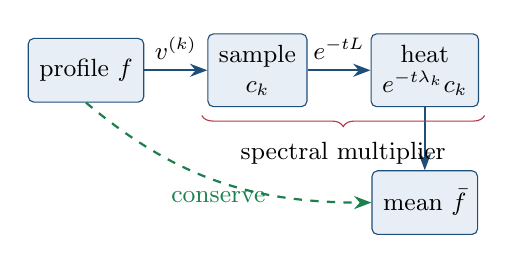
\begin{tikzpicture}[font=\small,
  box/.style={draw=sfblue,fill=sfink,rounded corners=2pt,inner sep=4pt,align=center,minimum height=2.3em},
  arr/.style={-{Stealth[length=2.2mm]},thick,draw=sfblue}]
  \node[box] (f) {profile \(f\)};
  \node[box,right=8mm of f] (s) {sample\\ \(c_k\)};
  \node[box,right=8mm of s] (h) {heat\\ \(e^{-t\lambda_k}c_k\)};
  \node[box,below=8mm of h] (m) {mean \(\bar f\)};
  \draw[arr] (f) -- node[above,text=black] {\(v^{(k)}\)} (s);
  \draw[arr] (s) -- node[above,text=black] {\(e^{-tL}\)} (h);
  \draw[arr] (h) -- (m);
  \draw[arr,dashed,sfgreen] (f.south) to[out=-40,in=180] node[below,text=sfgreen] {conserve} (m.west);
  \draw[decorate,decoration={brace,amplitude=4pt,mirror},sfred]
    ($(s.south west)+(-2pt,-3pt)$) -- ($(h.south east)+(2pt,-3pt)$)
    node[midway,below=6pt,text=black] {spectral multiplier};
\end{tikzpicture}
\caption{Sampling, the heat multiplier, and the conserved mean. Dashed arrow: the kernel of \(L\).}
\label{fig:flow}
\end{figure}

\section{A plot}
\label{sec:plot}
Figure~\ref{fig:gap} plots the gap \(\lambda_1(n)=4\sin^2(\pi/(2n))\) against its continuum stand-in \(\pi^2/n^2\), for \(n\) from 4 to 48. Both curves are smooth, the markers are filled, and the legend sits inside the axis. A viewer that substitutes a bitmap for the vector figure, or that drops the axis labels, is failing this page rather than the prose.

\begin{figure}[t]
\centering
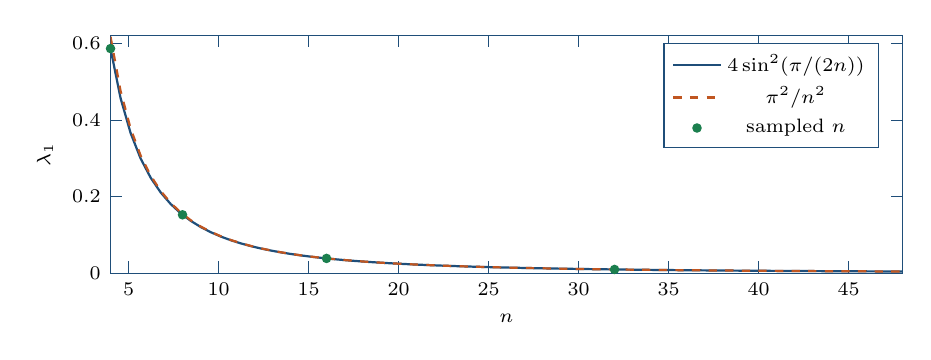
\begin{tikzpicture}
\begin{axis}[
  width=0.96\columnwidth,
  height=4.6cm,
  xlabel={\(n\)},
  ylabel={\(\lambda_1\)},
  xmin=4, xmax=48,
  ymin=0, ymax=0.62,
  tick label style={font=\scriptsize},
  label style={font=\scriptsize},
  legend style={font=\scriptsize,at={(0.97,0.97)},anchor=north east,draw=sfblue,fill=white},
  axis line style={sfblue},
  tick style={sfblue},
  every axis plot/.append style={line width=0.8pt},
]
\addplot[sfblue,domain=4:48,samples=80] {4*sin(deg(pi/(2*x)))^2};
\addlegendentry{\(4\sin^2(\pi/(2n))\)}
\addplot[sforange,domain=4:48,samples=80,dashed] {pi^2/(x^2)};
\addlegendentry{\(\pi^2/n^2\)}
\addplot[only marks,mark=*,mark size=1.3pt,sfgreen] coordinates {(4,0.5858) (8,0.1522) (16,0.0384) (32,0.0096)};
\addlegendentry{sampled \(n\)}
\end{axis}
\end{tikzpicture}
\caption{Spectral gap of the path versus the first Neumann eigenvalue of the interval, scaled by \(1/n^2\).}
\label{fig:gap}
\end{figure}

\section{A table}
\label{sec:table}
Table~\ref{tab:modes} lists the first four eigenvalues for three lengths of path, together with the relative gap \((\lambda_k-\pi^2 k^2/n^2)/(\pi^2 k^2/n^2)\). The header row is tinted; the body alternates. Negative relatives are expected: the discrete gap sits slightly below the continuum value once \(n\) is moderate, except at the coarsest grids.

\begin{table}[t]
\centering
\small
\begin{tabular}{@{}crrr@{}}
\toprule
\rowcolor{sfblue}
\textcolor{white}{\(n\)} & \textcolor{white}{\(\lambda_1\)} & \textcolor{white}{\(\lambda_2\)} & \textcolor{white}{rel.\ \(k{=}1\)} \\
\midrule
\rowcolor{sfpanel} 4  & 0.5858 & 2.0000 & \(+5.4\%\) \\
8  & 0.1522 & 0.5858 & \(+1.3\%\) \\
\rowcolor{sfpanel} 16 & 0.0384 & 0.1522 & \(+0.3\%\) \\
32 & 0.0096 & 0.0384 & \(+0.1\%\) \\
\bottomrule
\end{tabular}
\caption{Path Laplacian eigenvalues and the relative error of \(\lambda_1\) against \(\pi^2/n^2\).}
\label{tab:modes}
\end{table}

The same numbers written as a small aligned display, so a failed tabular does not hide the values:
\begin{align*}
\lambda_1(4)&=2-\sqrt{2},&
\lambda_1(8)&=2-\sqrt{2+\sqrt{2}},\\
\lambda_2(4)&=2,&
\lambda_2(8)&=2-\sqrt{2}.
\end{align*}

\section{Heat at a point}
\label{sec:heat}
Take \(n=8\) and the mean-zero bump \(f=(1,1,0,0,0,0,-1,-1)\). Its energy is
\begin{equation}
f^{\mathsf T}Lf = (1-1)^2+(1-0)^2+0+0+0+(0-(-1))^2+(-1-(-1))^2 = 2,
\end{equation}
and Claim~\ref{clm:gap} only says \(\|f\|_2^2=4\le \lambda_1^{-1}\cdot 2\). Since \(\lambda_1(8)\approx 0.152\), the constant \(\lambda_1^{-1}\approx 6.57\) clears \(4\) with room to spare; the inequality is not sharp on this vector because \(f\) is not the first sine mode.

The mode weights that do decay are the Fourier cosine coefficients against \(v^{(k)}\). Writing \(Z_k=\|v^{(k)}\|_2\),
\begin{equation}
c_k = Z_k^{-1}\sum_{j=1}^{n} f_j\cos\frac{(j-\tfrac12)k\pi}{n},
\qquad
|c_k|\,e^{-t\lambda_k}\ \text{is the height at time \(t\).}
\end{equation}
Figure~\ref{fig:decay} draws three of those envelopes. A log axis makes the gap visible: \(k=1\) is still above \(10^{-2}\) when \(k=3\) has already fallen through \(10^{-4}\).

\begin{figure}[t]
\centering
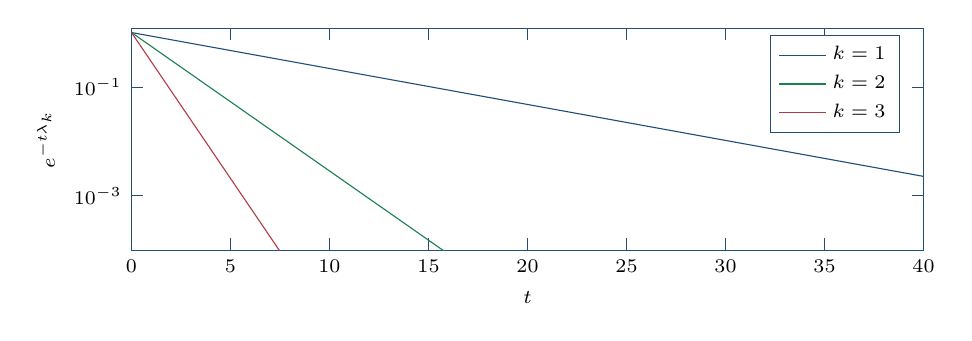
\begin{tikzpicture}
\begin{axis}[
  width=0.96\columnwidth,
  height=4.4cm,
  xlabel={\(t\)},
  ylabel={\(e^{-t\lambda_k}\)},
  xmin=0, xmax=40,
  ymin=1e-4, ymax=1.2,
  ymode=log,
  tick label style={font=\scriptsize},
  label style={font=\scriptsize},
  legend style={font=\scriptsize,at={(0.97,0.97)},anchor=north east,draw=sfblue,fill=white},
  axis line style={sfblue},
  tick style={sfblue},
]
\addplot[sfblue,domain=0:40,samples=60] {exp(-x*0.1522)};
\addlegendentry{\(k=1\)}
\addplot[sfgreen,domain=0:40,samples=60] {exp(-x*0.5858)};
\addlegendentry{\(k=2\)}
\addplot[sfred,domain=0:18,samples=40] {exp(-x*1.2346)};
\addlegendentry{\(k=3\)}
\end{axis}
\end{tikzpicture}
\caption{Decay of the first three positive modes on the path of length 8.}
\label{fig:decay}
\end{figure}

The same decay written without a picture, for a renderer that paints rules and not plots:
\begin{equation}
\begin{cases}
e^{-10\lambda_1}\approx 0.218, & \\
e^{-10\lambda_2}\approx 0.0028, & \\
e^{-10\lambda_3}\approx 4.3\times 10^{-6}. &
\end{cases}
\end{equation}

\section{What a viewer owes this file}
\label{sec:viewer}
The outline of this note has six entries, all of them destinations of the coloured cross-references above: Setup~\ref{sec:setup}, the calculation~\ref{sec:calc}, the diagram~\ref{sec:diagram}, the plot~\ref{sec:plot}, the table~\ref{sec:table}, and this section. A sidebar of page thumbnails should show a title page with a blue abstract box, a page dominated by display mathematics, and a page carrying the figure and the plot.

External link, left as a live URI annotation: \url{https://ctan.org/pkg/pgf}.
Internal jump: the spectrum is \eqref{eq:spectrum}, the decay is \eqref{eq:decay}, and the picture is Figure~\ref{fig:flow}.

\begin{claim}
A faithful rendering of this file shows Latin Modern italic in \(f^{\mathsf T}Lf\), a radical and a fraction bar in \eqref{eq:glyphs}, two colours of rule in Figure~\ref{fig:flow}, a dashed orange curve in Figure~\ref{fig:gap}, and a blue header row in Table~\ref{tab:modes}.
\end{claim}

\end{document}
